\documentclass[crop,tikz]{standalone}% 'crop' is the default for v1.0, before it was 'preview'
\usetikzlibrary{arrows.meta}
%\usetikzlibrary{...}% tikz package already loaded by 'tikz' option

\usepackage{bm}
\usepackage{xcolor}


\begin{document}
	\usetikzlibrary{arrows.meta}
	\begin{tikzpicture}[
		my node/.style={circle, black, fill = black!10!white, minimum size=30pt, inner sep=0pt, align = center},
		my arrow/.style={-Triangle}
		]
		\node[scale = 1.2] at (1.3, 1.25) {\textbf{Causal structure}};
		\node[my node] (X1) at (1.25,0) {$\bm{X_1}$};
		\node[my node] (X4) at (0,-2.625) {$\bm{X_4}$};
		\node[my node] (X2) at (2.5,-1.75) {$\bm{X_2}$};
		\node[my node] (X3) at (2.5,-3.5) {$\bm{X_3}$};
		\node[my node] (X5) at (2.5, -5.5) {$\bm{X_5}$};
		\node[my node, fill = black!30!white] (Y) at (0.5,-5) {$\bm{Y}$};
		
		\draw[my arrow] (X1) -- (X4);
		\draw[my arrow] (X1) -- (X2);
		\draw[my arrow] (X2) -- (X3);
		\draw[my arrow] (X4) -- (Y);
		\draw[my arrow] (X3) -- (Y);
		\draw[my arrow] (X3) -- (X5);
		
		% Include image
		\node at (14.2, -2.4) {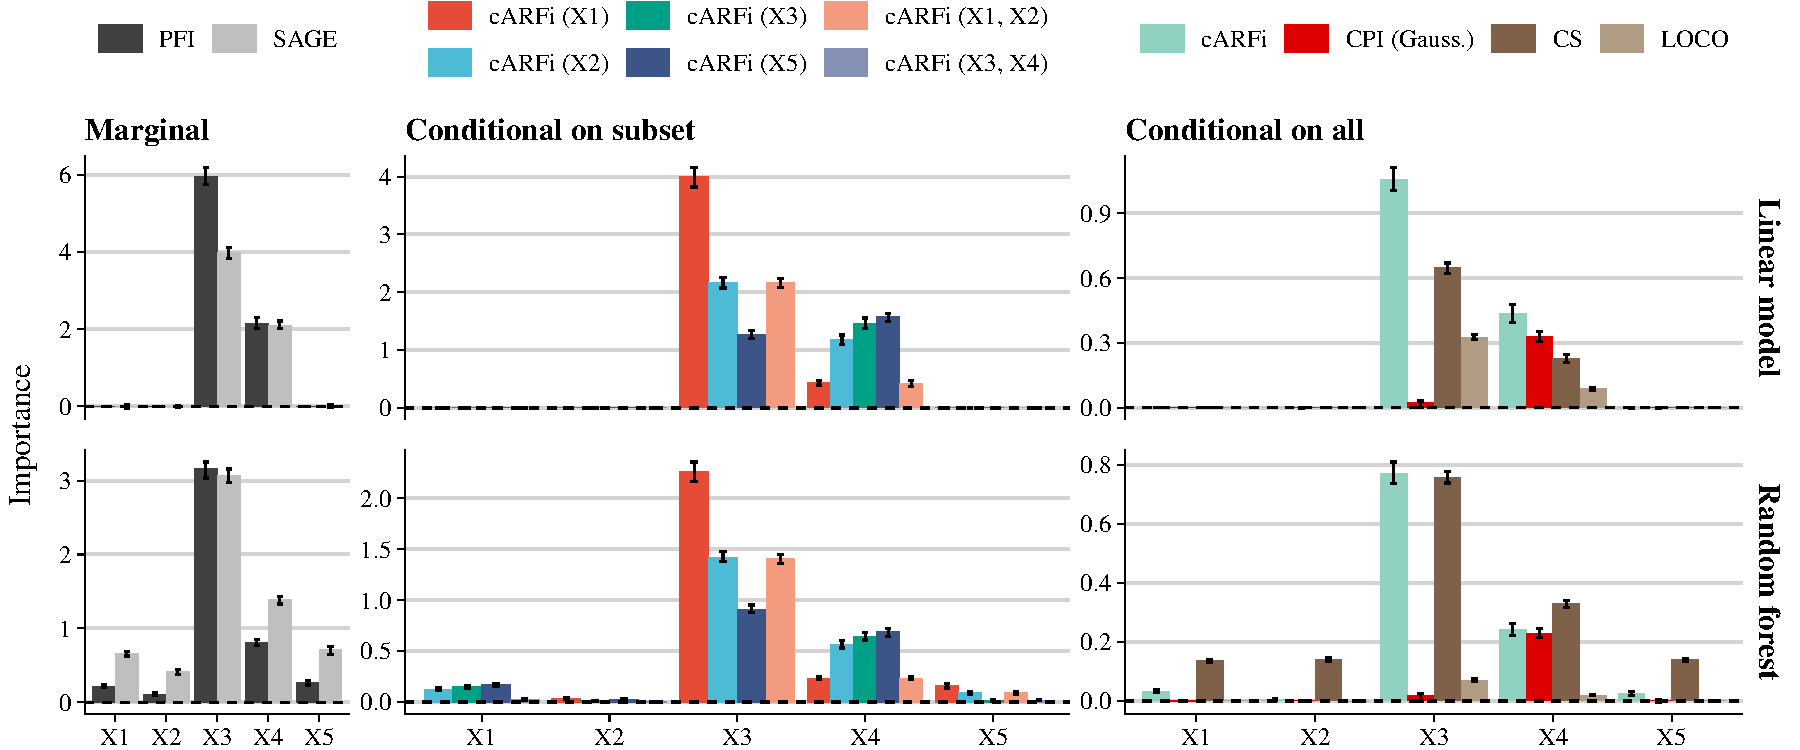
\includegraphics[scale = 0.7]{figures/plot_conditioning_set.pdf}};
		
	\end{tikzpicture}
\end{document}